\section{Sobre o modelo em \LaTeX}

Este documento e seu código-fonte formam o modelo \LaTeX\ de artigo para TCC no IFRS \textit{campus} Rolante. Ele é baseado nos pacotes \abnTeX\ e \textsf{abntex2cite}. O documento exemplifica a elaboração de publicação periódica científica impressa produzida conforme a ABNT NBR 6022:2018 \emph{Informação e documentação - Artigo em publicação periódica científica - Apresentação}. Uma lista completa das normas observadas pelo \abnTeX\  é apresentada em \citeonline{abntex2classe}.

Faça upload deste modelo (com todos os seus arquivos) no \href{https://overleaf.com/project}{overleaf}, um  serviço gratuito e online de edição e compilação de arquivos \LaTeX. Alternativamente, faça uso de um editor offline (como o \texttt{texmaker} ou o \texttt{textstudio}), ou utilize um plugin para sua IDE preferida (como o \LaTeX Workshop para o Visual Studio).

\subsection{Exemplos}

\subsubsection{Citações}

Os seguintes tipos de citações são definidos na NBR 10520 \cite{NBR10520:2002}.

\begin{itemize}
	\item \textbf{Citação direta}: ``Transcrição textual de parte da obra do autor consultado'' \cite{NBR10520:2002};
	\item \textbf{Citação indireta}: A citação indireta não recebe aspas, porém é baseada na obra do autor consultado \cite{NBR10520:2002}.
\end{itemize}

No \LaTeX\ uma citação direta com menos de três linhas deve ser iniciada com duas crases e finalizada com duas aspas simples. O \LaTeX\ renderizará esses elementos no PDF como abertura e fechamento de aspas duplas estilizadas adequadamente.

Por fim, o pacote \abnTeX fornece uma estrutura para fazer citações diretas com mais de três linhas. Por exemplo:

% Exemplo de citação direta com mais de 3 linhas e
\begin{citacao}
	Lorem ipsum dolor sit amet, consectetuer adipiscing elit. Ut purus elit, vestibulum ut, placerat ac, adipiscing vitae, felis. Curabitur dictum gravida mauris. Nam arcu libero, nonummy eget, consectetuer id, vulputate a, magna. Donec vehicula augue eu neque. Pellentesque habitant morbi.
 \end{citacao}

\subsubsection{Referências}

Talvez o maior pesadelo dos pesquisadores iniciantes em \LaTeX\ seja organizar e adequadamente formatar referências em seus artigos. O \LaTeX\ além de formatar o texto, também formata as referências. Para isso, você precisa listar as informações que identificam/descrevem os trabalhos que queres referenciar. Isso deve ser feito no arquivo \texttt{referencias.bib} seguindo um formato pré-determinado. No final do arquivo \texttt{main.tex} o comando \verb|\bibliography{referencias}| é responsável por informar ao pacote \abnTeX\ que é nele que estão listadas as referências. Dependendo do compilador \LaTeX\ utilizado, talvez seja necessário compilar o \texttt{main.tex} mais do que uma vez até que as referências sejam atualizadas (ou compiladas pela primeira vez).

Abra o arquivo \texttt{referencias.bib}, veja os exemplos e com base neles aprenda como criar suas próprias referências. Este formato é chamado de BibTeX.

Informação bônus: o google scholar gera o código BibTeX de artigos e livros. Ou seja, ao encontrar um trabalho que deseja referenciar em seu artigo no google scholar, basta clicar no link ``Cite'' e então no link ``BibTeX'' e será apresentado com o respectivo código BibTeX. Atenção, nem sempre o google scholar incluirá o DOI do artigo, ou o ISBN no caso de livros. É natural que você precise adicionar essas informações manualmente.

\subsubsection{Figuras}

Figuras/imagens devem ser, idealmente, vetoriais. Imagens vetoriais não descrevem cores de pixels, mas sim formas geométricas. O leitor PDF interpreta estas imagens e as mostra sem a inclusão de borrados, sombras ou outros problemas. 

Use ferramentas como o \href{https://draw.io}{draw.io} para criar desenhos, fluxos, diagramas, e etc em formato vetorial. Basta exportar sua figura no formato PDF e usar alguma ferramenta para remover as bordas do PDF como o \href{https://pdfresizer.com/crop}{pdfresizer}. Isso é necessário pois geralmente a exportação em PDF será feita no formato A4 para impressão. Por fim, inclua e faça referência da imagem no seu texto conforme o exemplo abaixo. Lembre-se, toda Figura deve ser referenciada e explicada no texto. Por exemplo, a Figura~\ref{fig1} mostra um fluxograma.

\begin{figure}[h]
	\centering
	\label{fig1}
	\caption{Exemplo de figura vetorial.}
	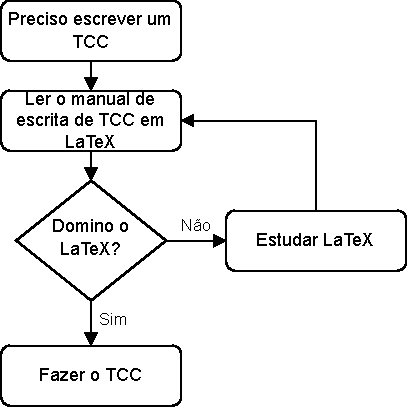
\includegraphics[width=0.5\textwidth]{figuras/diagrama-tcc-latex.pdf}
	\fonte{Elaboração própria.}
\end{figure}

Muitos alunos tem dificuldade em posicionar imagens e tabelas em \LaTeX. O \verb|[h]| no \verb|\begin{figure}[h]| indica que o autor deseja que o \LaTeX\ posicione a imagem tal como está no texto. Substituindo por \verb|[t]| indicamos que desejamos no topo da página, o que geralmente resulta na imagem sendo incluída no topo da próxima página. Por fim, se o \verb|[h]| for insuficiente, use o \verb|[H]| para obrigar o \LaTeX\ a posicionar a imagem tal como no seu código-fonte. Cuidado, isso pode gerar problemas!

Para controlar o tamanho da figura, altere o multiplicador \verb|0.5| no comando \verb|\includegraphics[width=0.5\textwidth]|. Isso controla a largura da imagem. A altura é ajustada com base na largura automaticamente.

Todas as figuras e tabelas devem ter sua breve descrição na parte superior e a indicação de autoria na parte inferior.

\subsubsection{Tabelas}

A criação de tabelas no \LaTeX\ é uma arte. De início, use sites como o \href{https://www.tablesgenerator.com/}{tablesgenerator.com}. Nele você graficamente desenha a tabela que deseja e ele gerará o código \LaTeX. As regras gerais são não criar linhas separadoras verticais, apenas horizontais para delimitar o início da tabela, o cabeçalho, e o fim da tabela. Apenas use linhas horizontais no meio da tabela quando estritamente necessário. Por exemplo, como foi feito na Tabela~\ref{tbl1}. Sempre use sempre as opções do pacote \verb|booksmark| (incluído pelo \abnTeX\ por padrão) para as separações horizontais. São elas o \verb|\toprule| para início, o \verb|\midrule| para o fim do cabeçalho e eventuais linhas horizontais no meio da tabela e \verb|\bottomrule| para o fim da tabela.

\subsubsection{Equações}

Evite equações \textit{in line}, ou seja, dentro do texto. A preferência sempre deve ser por equações definidas com o \verb|\begin{equation}|, de forma que as equações sejam numeradas e que você possa referenciá-las no texto. Por exemplo, veja a Equação~\ref{eq1}:

\begin{equation} \label{eq1}
	a^2 = b^2 + c^2
\end{equation}

Também é possível alinhar as com o ambiente \verb|\begin{split}| fazendo uso do \verb|&| como indicador de alinhamento. Veja um exemplo de equações alinhadas na Equação~\ref{eq2}.

\begin{equation} \label{eq2}
	\begin{split}
	A & = \frac{\pi r^2}{2} \\
	 & = \frac{1}{2} \pi r^2
	\end{split}
\end{equation}

Uma lista abrangente de símbolos matemáticos está disponível \href{https://oeis.org/wiki/List_of_LaTeX_mathematical_symbols}{aqui}.
